\section{Controllers Implementation}
The implementation of the controllers can not be done having them as a continuous expression due to the discrete operation of the microcontroller. 

In order to discretize the controllers in the system, they need to be expressed in terms of the $z$ operator, the equivalent to the Laplace operator in the discrete domain. This transformation is done through the Tustin (bilinear) approximation in which the $s$ term in the transfer function is substituted as seen in \autoref{tustin} \cite{tustin}.
\begin{flalign}
	s\approx\frac{2}{T}\frac{z-1}{z+1}
	\label{tustin}
\end{flalign}
\begin{where}
	\va{s}{is the Laplace operator}{}
	\va{z}{is the discrete operator}{}
	\va{T}{is the sampling time}{}
\end{where}
The Tustin approximation maps the Laplace stable region into the discrete stable region, that is, the unit circle, as seen in \autoref{fig:tustinmap}. For these reason, is one of the most used discretization methods.
\begin{figure}[H]
	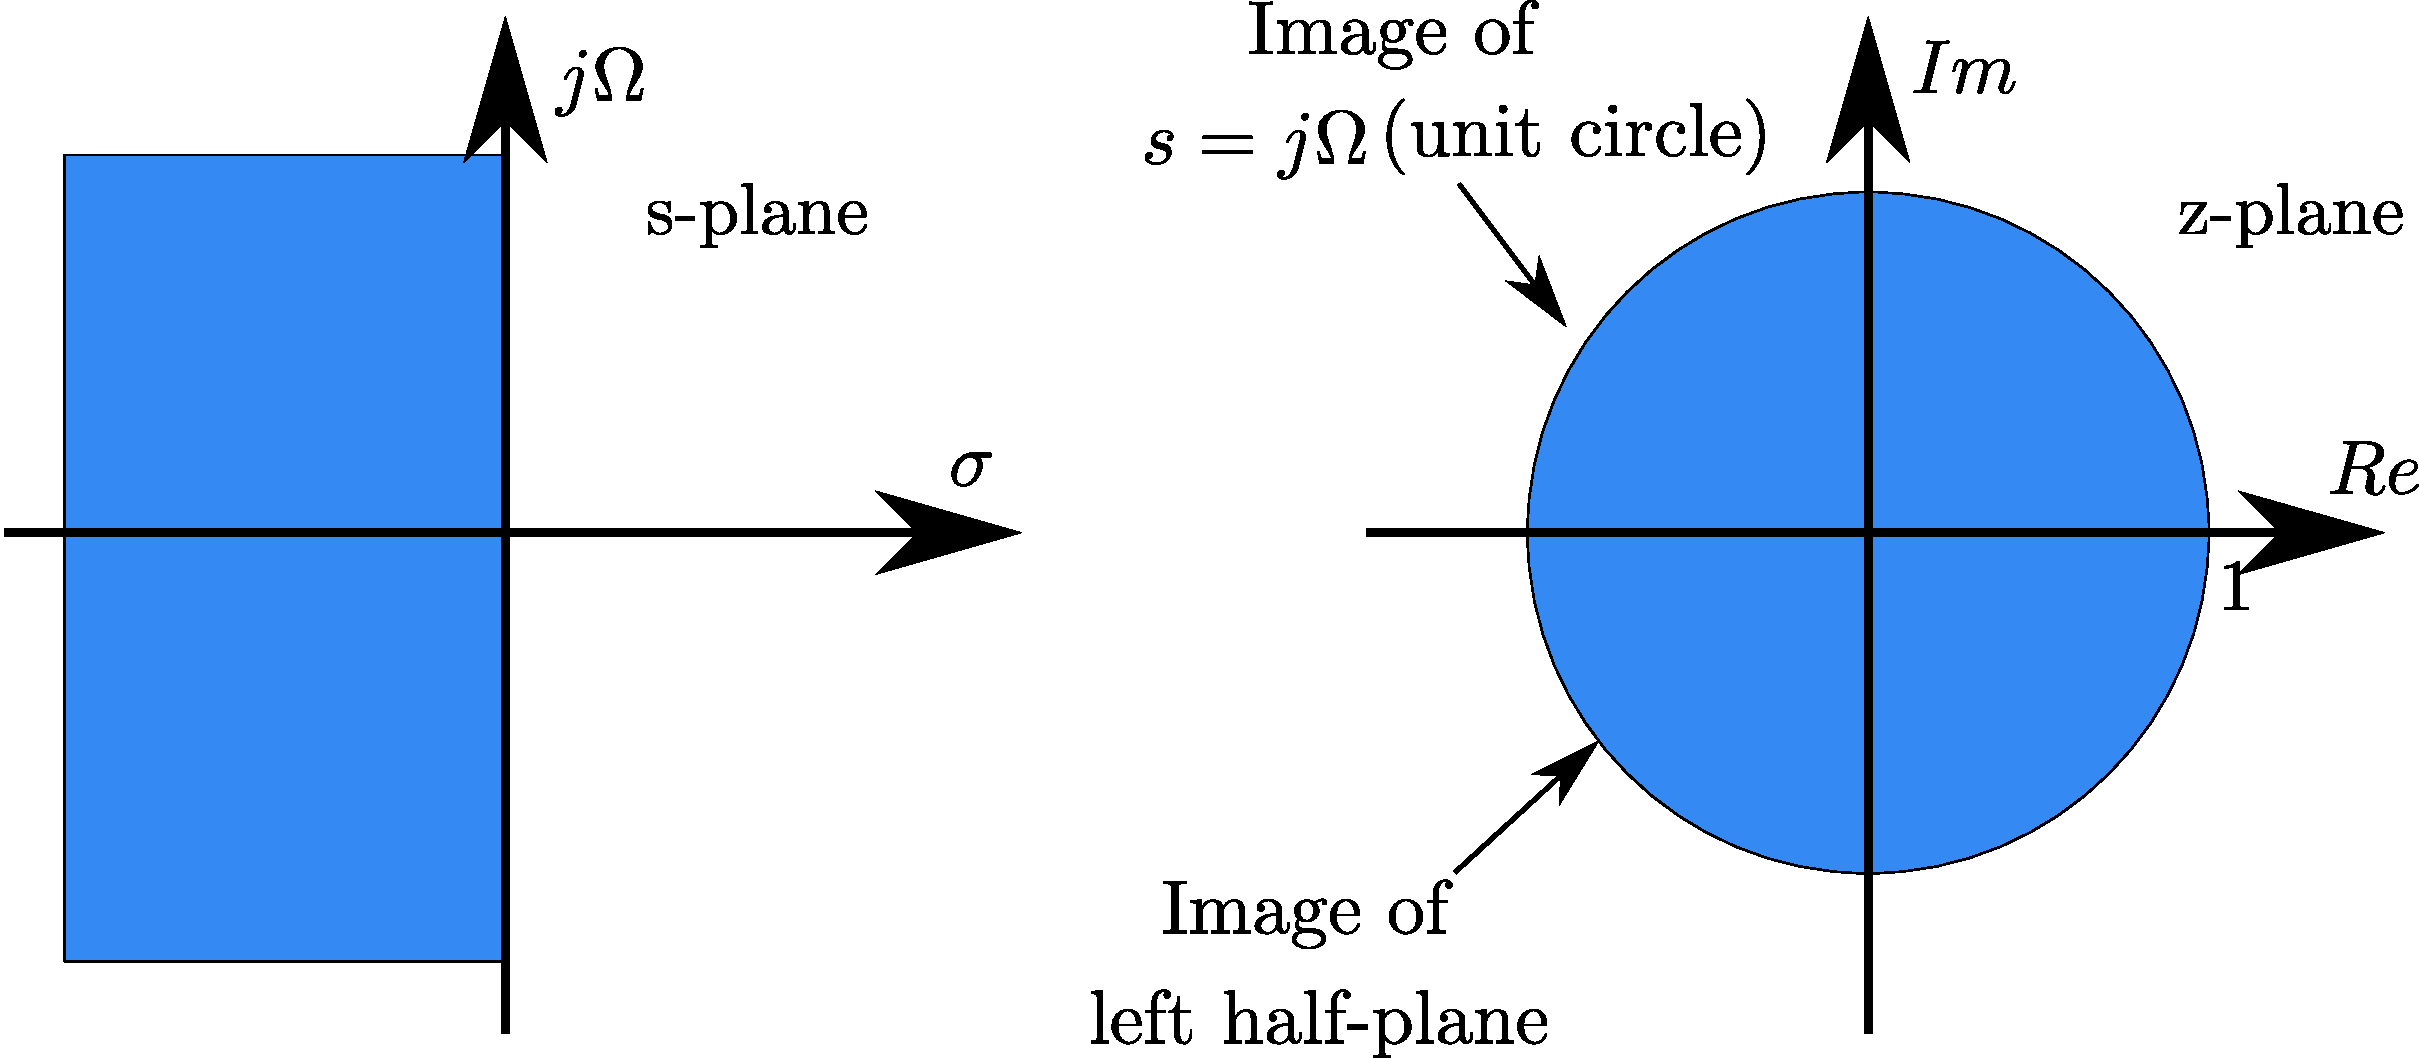
\includegraphics[scale=.3]{figures/SplaneVsZplane.pdf}
	\centering			
	\captionof{figure}{The s-domain and the z-domain \cite{AVOppenheim}.} 
	\label{fig:tustinmap}
\end{figure} 
The discrete transfer function is then transformed into a difference equation to obtain the expression to be applied in the microcontroller. This is done taking into account that a $z^{-1}$ term implies taking the previous sample of the data. 

When discretizing the controller, the sampling time must also be considered. In the system at hand, the sampling frequency is limited by the sensor data (Vicon System) to be 100 Hz as a maximum. The lower limit comes from the bandwidth of the controllers as for the discretization not to affect the controller response, the sampling frequency should from 10 to 20 times higher than the bandwidth of the control loop. The fastest control loop in the system is the attitude controller and has a bandwidth of 5 rad/s, that is, 0.8 Hz. This implies a minimum sampling frequency of 20 Hz.\fxnote{CHECK NUMBERS}

The chosen sampling frequency in the system is 28 Hz in order to keep the controllers with a good performance an far from the 100 Hz that Vicon provides in order to have time for processing the communication and the control tasks.\fxnote{CHECK NUMBERS}

\subsection{Attitude Controllers}
The attitude controller is mainly composed of gains formed by the state feedback, the integral and the observer matrices. this makes the discretization easier as there are no $s$ terms in the controller. There are though two integrators, one is in the observer and the other one is placed in the integral term of the controller.

The discrete form of an integrator using the bilinear approximation is shown in \autoref{discreteIntegrator}. The formula shows how the integrator in the integral term of the attitude control looks like when discretized.  
\begin{flalign}
	\frac{x_{int}}{\phi_{ref}-\phi}=\frac{x_{int}}{e_{\phi}} \approx \frac{T}{2}\frac{z+1}{z-1}
	\label{discreteIntegrator}
\end{flalign}
This transformation yields a difference equation as seen in \autoref{discreteIntegratordifferences}, which shows the example in the roll angle case. It gives the current value of the integral state as a function of the previous integral state and the current and the previous error between the angular reference and the angular data.
\begin{flalign}
	x_{int}(k)=x_{int}(k-1) + \frac{T}{2} e_{\phi}(k) + \frac{T}{2} e_{\phi}(k-1)
	\label{discreteIntegratordifferences}
\end{flalign}

The effect of the discretization in the designed attitude controllers has been simulated in the non-linear system and it is commpared with the continuous designed previously developed. See \autoref{fig:AttitudeDiscrete}. It can be seen that the discretized version of the controller makes it slower, but the overshoot is slightly reduced. There no change in the final value of the controller.
\begin{figure}[H]
	\centering
	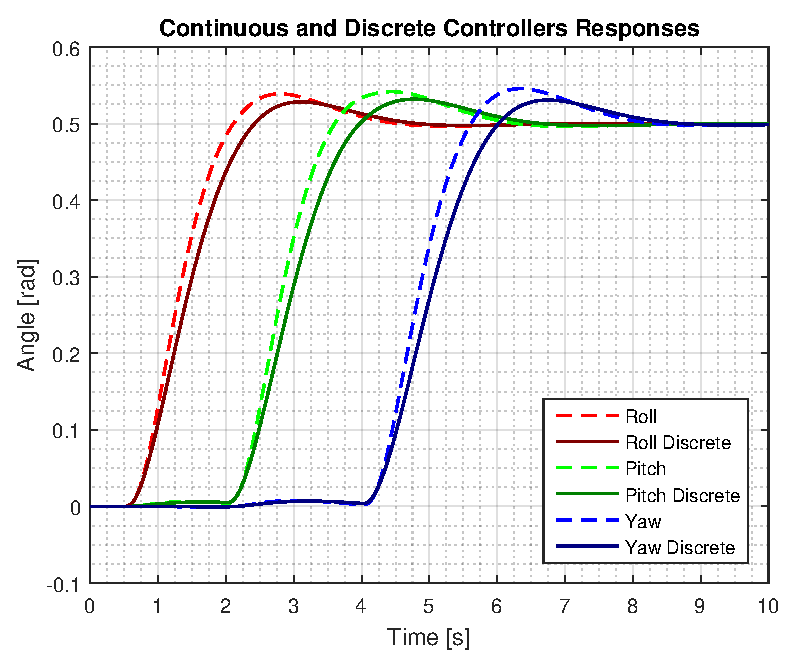
\includegraphics[scale=0.65]{figures/simAttitudeDiscrete}
	\caption{Attitude controller performance when discretized with a sampling rate of 28 Hz and its continuous version.}
	\label{fig:AttitudeDiscrete}
\end{figure}

The discrete attitude controller is also evaluated by its control action, which is depicted in \autoref{fig:AttitudeDiscreteControlAction}. As it can be appreciated, the variations from equilibrium of the motor rotational speeds are larger in the discrete controller and the signals are away from equilibrium for a longer time.
\begin{figure}[H]
	\centering
	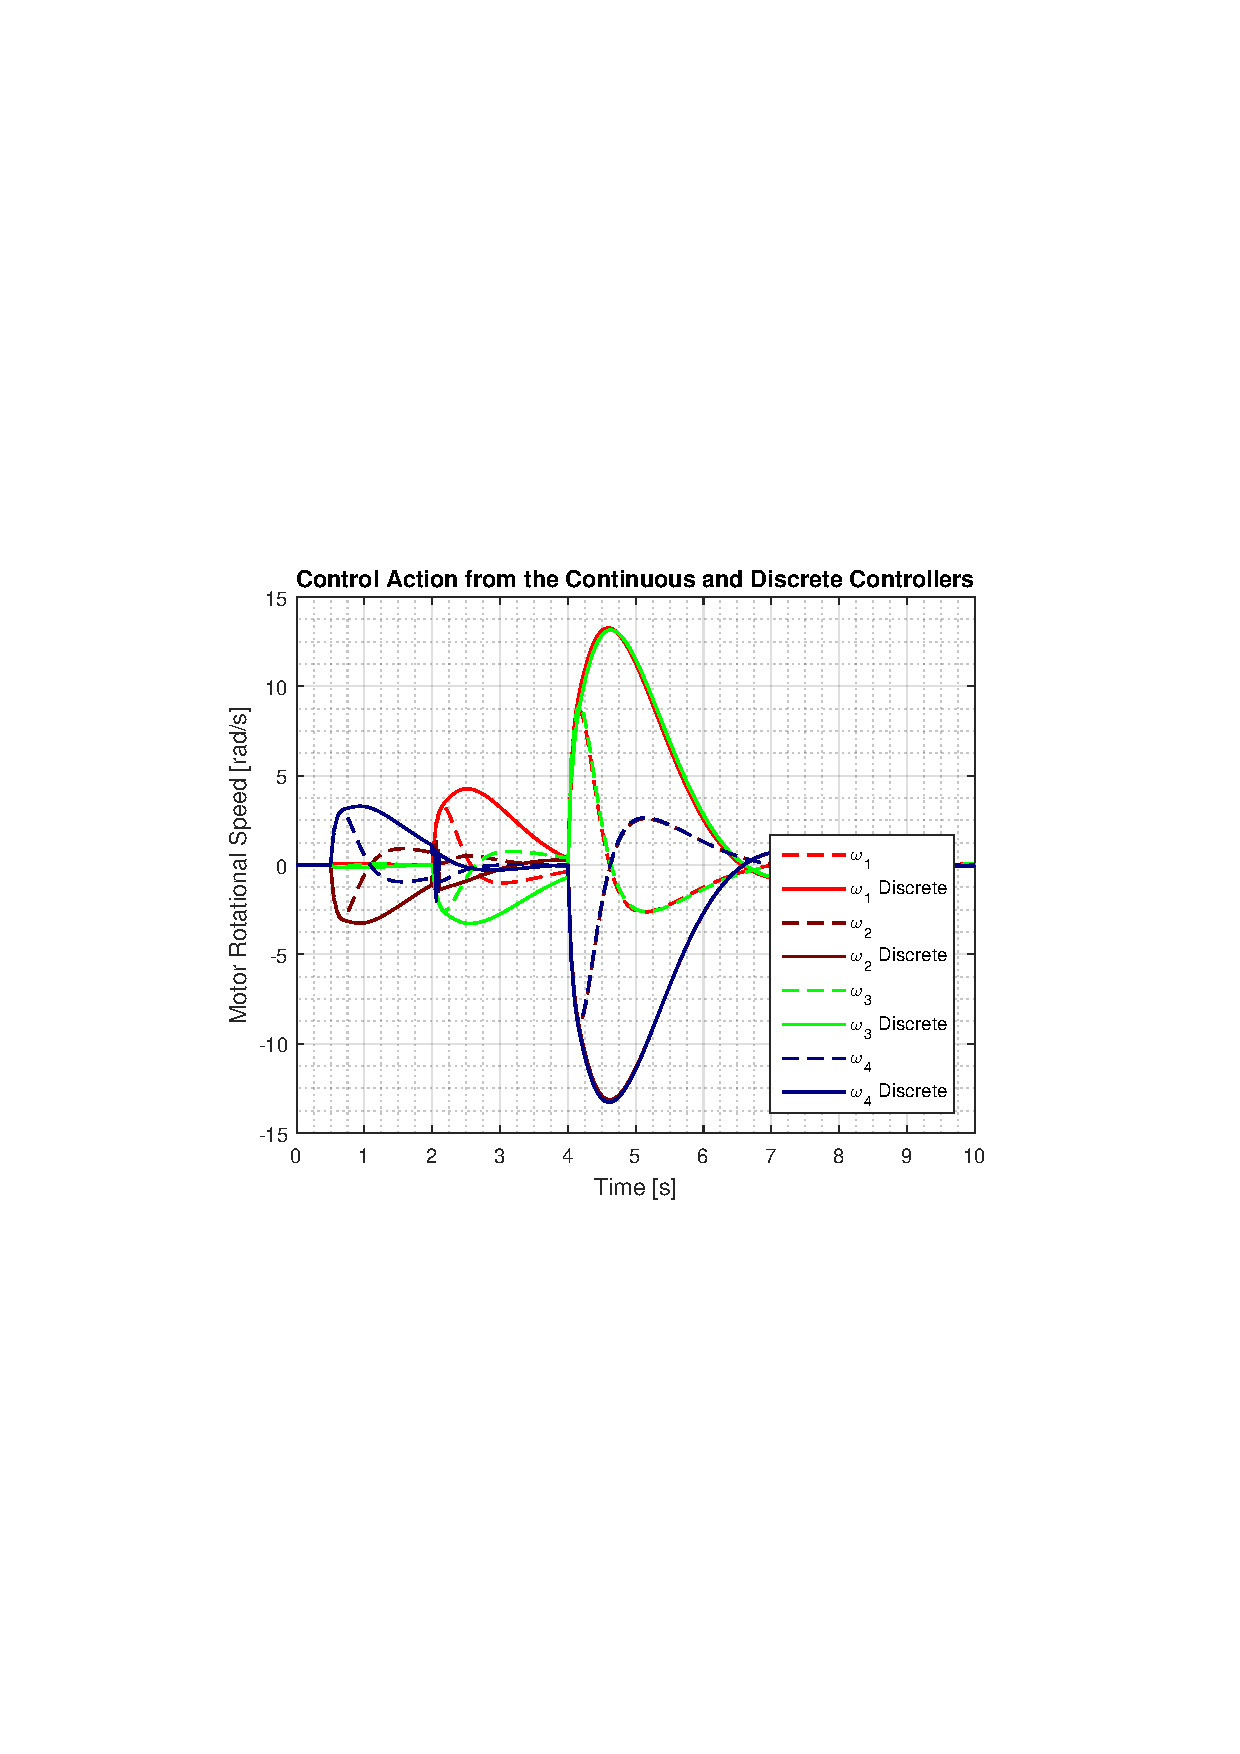
\includegraphics[scale=0.65]{figures/simAttitudeDiscreteControlAction}
	\caption{Attitude controller control action when discretized with a sampling rate of 28 Hz and its continuous version.}
	\label{fig:AttitudeDiscreteControlAction}
\end{figure}
 
\subsection{Translational Controllers}
The translational controllers are all proportional controllers except the velocity z controller, which is a PI controller. The gains are the same in both continuous and discrete domains but the PI needs to be discretized with the Tustin rule. 

The discrete version of the z controller is shown in \autoref{discreteVelocityZcontroller}.
\begin{flalign}
	\frac{\omega_{sum}}{e_{\dot{z}}} = tf_{cont} \approx tf_{discrete}
	\label{discreteVelocityZcontroller}
\end{flalign}

From the above equation, the difference equation that should be implemented in the microcontroller is calculated. The final equation is shown in \autoref{discreteVelocityZcontrollerdiferences}. \fxnote{CHECK NUMBERS IN THE EQUATIONS}

\begin{flalign}
	\omega_{sum}(k)= \omega_{sum}(k-1) + e_{\dot{z}}(k) + e_{\dot{z}}(k-1)
	\label{discreteVelocityZcontrollerdiferences}
\end{flalign}

In \autoref{fig:} the comparison of the translational controllers discrete and continuous versions. In the simulation, only the sampling rate effect is taken into account. 
\begin{figure}[H]
	\centering
	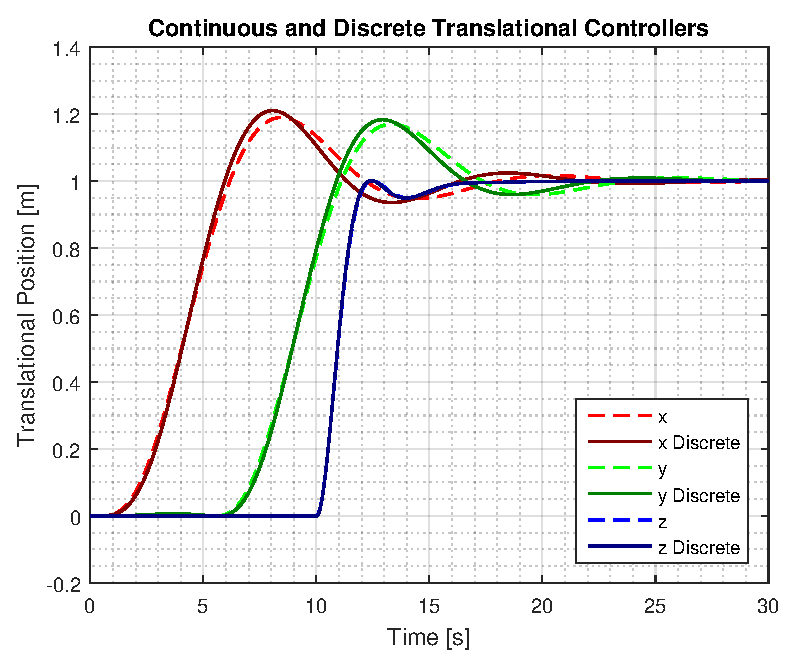
\includegraphics[scale=0.65]{figures/simTranslationalDiscrete}
	\caption{Translational position controller when discretized with a sampling rate of 28 Hz and its continuous version.}
	\label{fig:TranslationalDiscrete}
\end{figure}
The response of the controller becomes slower in both the x and y cases, in which the overshoot is also slightly reduced this is due to the effect of the sampling in the inner attitude controllers, see \autoref{fig:AttitudeDiscrete}, rather than on the translational controllers themselves as they are slow compared to the sampling rate of the system. In the z controller there is no noticeable differences between continuous and discrete versions as the sampling rate is fast compared with the controller.\fxnote{Include control action figure}